\section{Condition monitoring}
All rotating machinery eventually fails because of the long-term strain on the individual parts or incorrect workmanship, installation, or operational procedures. In the end, these factors cause the equipment not to fulfill its intended functionality. Many instrumentation methods are practiced to reveal evolving faults: vibration and acoustic noise monitoring, electric supply line measurements, thermography, oil and particle analysis, ultrasonic testing, etc. Vibration signals are the preferred tool for rotating machinery monitoring \cite{mohanty_machinery_2015}. 

The defect needs to be either repaired or replaced, preferably without significant production downtime, further damage to the other attached elements, or endangerment of the responsible personnel. The maintenance strategies are chosen according to the machine's importance as a result of its failure effect evaluation on the system. The guide to set appropriate maintenance procedures is outlined by IEC 60706-2 standard and involves reliability-centered maintenance (RCM) analysis \cite{el-thalji_predictive_2019}.

\subsection{Maintenance strategies}
There are three different approaches to maintenance across the industry: reactive, preventive, and predictive \cite{scheffer_practical_2004}. In general, the more sophisticated methods are beneficial in a high-stakes environment. The unexpected machine shutdown can have a negative economic impact on the enterprise, resulting in decreased product quality and demands spare parts be ready in the supply inventory at all times. However, in certain situations suffice to utilize a simpler maintenance program, but predictive maintenance gains interest in the Industry 4.0 to optimize usage of assets \cite{cinar_machine_2020}.

\paragraph{Reactive maintenance} allows machinery to run to complete failure. This is the most inefficient way to maintain the production line. It requires a large stock of replacement parts on-site and breakage constitutes a `crisis management mode' in the plant \cite{scheffer_practical_2004}. On-demand repairs are justified for consumer products or in the factory capable of fully and quickly replacing the halted machine with a backup. 

\paragraph{Preventive maintenance} is performed before any issue is detected. Maintenance occurs at regular intervals derived from a predetermined period in the calendar or expected machine running time (e.g. MTTF - Mean Time To Failure). The schedule is crucial but can result in components being replaced in good condition when further utilization is possible or too late after the machine breaks. In this case, conservative planning is usually the norm to keep machine always in perferct state which means more frequent intervention. \cite{mohanty_machinery_2015}.  

\paragraph{Predictive maintenance} known as condition-based (CbM), improves the predictability of reactive maintenance and eliminates the waste in overall resource utilization of cautious prevention. The machine downtime is scheduled after the detection of unhealthy trends in fault monitoring with sensors and troublesome components are identified. This allows us to order necessary parts in advance and organize repairs of several machines at a convenient time. The misdetection leads to increased costs compared to previous methods and raises the expectation that faults are distinguishable among themselves. \cite{davies_handbook_2012}. \\

\begin{figure}[h]
	\centering
	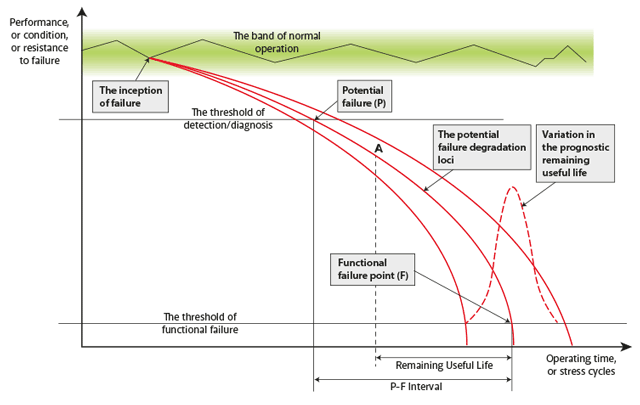
\includegraphics[width=\textwidth]{assets/P-F-Curve.png}
	\caption{P-F curve represets evolution of the asset's health \cite{jennions_integrated_2011}}
	\label{fig:p-f-curve}
\end{figure}

The P-F curve is a widespread representation of equipment degradation over time based on historical records (Fig.~\ref{fig:p-f-curve}). Corrective action should be taken between the event of potential failure (P), when the fault detection is activated, and functional failure point (F) in the P-F interval \cite{bousdekis_enterprise_2021}.  These division points are not exactly set but have statistical distribution to them.

The Remaining Useful Life (RUL) of the specific running machine in the given instance can be merely estimated analytically, with the survival probabilities of the individual components, and based on the model of the `run-to-failure' logs and usage parameters \cite{okoh_overview_2014}. Predictive condition monitoring aims to extend the machine lifespan to the maximum by predicting expected RUL.

The high failure rate is present not only when the part is worn out, but also in the early stages soon after assembly. Explanations range from inadequate installation to flimsily manufactured electrical or mechanical elements. The time plot to failure rate is known as the bath tub curve (Fig.~\ref{fig:bath-tub-curve}).

\begin{figure}[h]
	\centering
	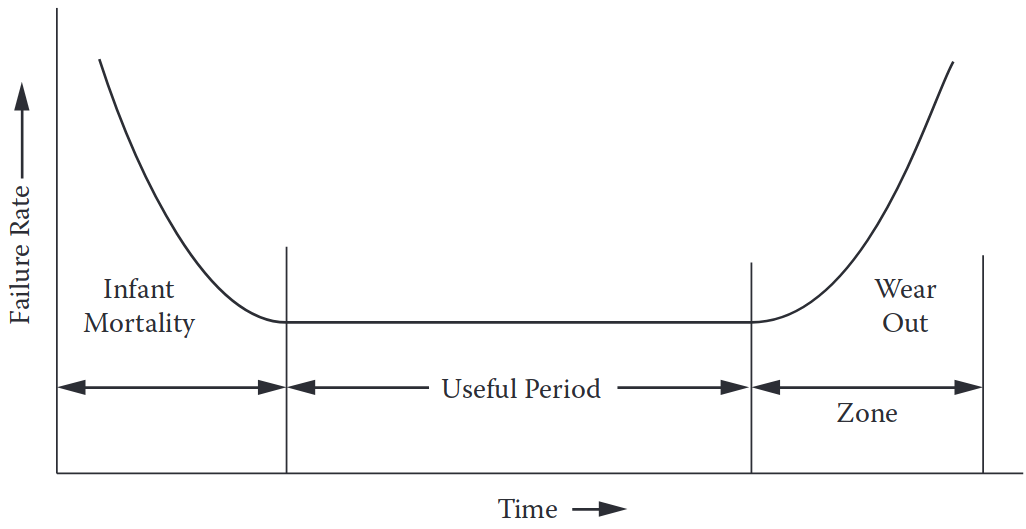
\includegraphics[width=0.9\textwidth]{assets/bath-tub-curve.png}
	\caption{Bath tub curve \cite{mohanty_machinery_2015}}
	\label{fig:bath-tub-curve}
\end{figure}

%TODO
\subsection{Vibration fault types}
\cite{scheffer_practical_2004} p.98 - 141

\cite{davies_handbook_2012} p.282
% Automatic Anomaly Detection in Vibration Analysis Based on Machine Learning Algorithms
\cite{torres_automatic_2022}
% Vibration Guide
\cite{noauthor_vibration_2000}
% The experimental application of popular machine learning algorithms on predictive maintenance and the design of IIoT based condition monitoring system
\cite{cakir_experimental_2021}
% Technická diagnostika
\cite{ziaran_technicka_2013}

Why monitor with vibrations,
- frequency ranges 1 - 300 Hz (shaft), 300 - 1000 Hz, 1000 - 10000 Hz (early bearings)
- Base analytical models: Jeffcott rotor - rotor dynamics, Bearnings model
- Resonance frequencies of each part - machine must run at speeds not aligned with resonance frequencies - Campbell diagram - task for mechanical engineers
- Faults - reasons and frequency content


\begin{itemize}
\item Synchrounous response - based on RPM
\item Mass unbalance
\item Misalignment
\item Eccentricity
\item Bent or bow shaft
\item Cracked shaft
\item Rotor rubs - friction
\item Looseness
\item Auxiliery mechanical systems: Gearbox, Bearings, Belt 
\end{itemize}

% Bandsaws
% Vibration of bandsaws
\cite{lengoc_vibration_1990}
% Study on Online Detection and Fault Diagnosis of Band Saw Equipment
\cite{chen_study_2014}

\subsection{Technical standards}
\paragraph{ISO 20816}
% ISO 20816-1:2016 - Mechanical vibration - Measurement and evaluation of machine vibration - Part 1: General guidelines
\cite{noauthor_iso_2016}
Part 1
\begin{itemize}
\item Measurement units - displacement, velocity, acceleration
\item RMS, and max. amplitude = severity
\item Measurement points for sensors (axial, radial) - image, and 45 degrees
\item Evaluation zones - A, B, C, D - Severity chart (Annex B) - Degradation model
\item Opeartional limits - Alarm, Trips
\end{itemize}

\paragraph{ISO 13373}
% ISO 13373-1:2002 - Condition monitoring and diagnostics of machines - Vibration condition monitoring - Part 1: General procedures
\cite{noauthor_iso_2016}
% ISO 13373-2:2016 - Condition monitoring and diagnostics of machines - Vibration condition monitoring - Part 2: Processing, analysis and presentation of vibration data
\cite{noauthor_iso_2016-1}

\cite{jack_d_frequency_nodate}
\begin{itemize}
\item Sensor mount type in relation to sensor resonance
\item Data presentation - standard display formats for analysis - trends, watefall plots ...
\item Potencial causes for faults (p. 45) - use in vibration fault types
\end{itemize}
 
